\documentclass{book}

\usepackage{pgfplots}
\usepackage{tikz}
\usepackage[]{xcolor}
\usepackage[english]{babel}
\usepackage[outline]{contour}

% Package to introduce the mapping cylinder PDF
\usepackage{pdfpages}

\usepackage{mathtools}
% mathtools is required for \coloneqq
% \usepackage{asymptote}
% \usepackage{asypictureB}

\pgfplotsset{compat=1.13}

\newcommand{\uint}{[0,1]}
\newcommand{\cartprod}{\times}
\newcommand{\suchthat}{\mid}
\newcommand{\realset}{R}
\newcommand{\naturals}{N}
\newcommand{\integers}{Z}
\newcommand{\isdefined}{\coloneqq}
\begin{document}
% \chapter{Motivation}
\chapter{Mathematical introduction}
% \section{Symbols}
% \begin{list}{$\bullet$}{}
%  \item $I$ means the \textbf{unit interval}, defined to be the closed interval $[0,1]$. Or, in other words, the set of real numbers which are greather than or equal to
%  zero and less than or equal to one;
%  \item $X = \{ \ldots \}$ we describe the elements of the set $X$ by what is inside the curly brackets (extensional definition);
% \end{list}
\section{Topology preliminaries}
\subsection{Open sets}
\textit{\textbf{Open sets} are defined as being the sets belonging to a family $\tau$, if $\tau$ is a topology on $X$. $\tau$, in its turn, is a \textbf{topology} on
$X$ if the following list of requirements is satisfied:
\begin{list}{$\bullet$}{}
 \item $X \in \tau$ and $\emptyset \in \tau$. Both the empy set and $X$ are in $\tau$;
 \item $\{O_i\}_{i \in I} \subseteq \tau \implies \bigcup_{i \in I} O_i \in \tau$. If the family of all $O_i$ (with $i$ in a arbitrary index set) is a subset of the family
 $\tau$, then every union of the subsets $O_i$ is also a subset in the family $\tau$;
 \item $\{O_i\}_{i=1}^{n} \subseteq \tau \implies \bigcap_{i=1}^{n} O_i \in \tau$. If the family of all $O_i$ (with $i$ in a finite set) is in the family $\tau$, then
 every (consequently) finite union of the subsets $O_i$ is also a subset in the family $\tau$.
\end{list}
}
% 
\subsection{Image of a function and inverse image}
% A subset $A$ of $X$, has its image on a function $f$ defined by
% \begin{equation}
% %   f(A) = \{f: A \to X, \text{if for every a there exists an} x \in X, \text{such that} f(a) = x\}.
% \end{equation}

\subsection{Continuous functions}
\textit{A function $f: X \to Y$ is said to be \textbf{continuous} if for every open set $W \subseteq Y$, the inverse image of $f$
\begin{equation}
 f^{-1}(W) = \{x \in X \suchthat f(x) \in W\}
\end{equation}
is an open subset of $X$.}
% 
\subsection{Homeomorphism}
\textit{A \textbf{homeomorphism} is a continuous bijective function between topological spaces that has a continuous inverse function.}
Homeomorphism are the isomorphism in the category of topological spaces. They are the mappings that preserve \textit{all} topological properties of a given space.

A function $f: X \to Y$ between topological spaces $X$ and $Y$ is a homeomorphism if
\begin{list}{$\bullet$}{}
 \item $f$ is continuous;
 \item $f$ is a bijection ($f$ maps every element of $X$ into only one element of $Y$, and no element of $Y$ is ``unmapped'');
 \item $f^{-1}$ is continuous.
\end{list}

That is why homeomorphism are sometimes called \textbf{bicontinuous functions}. \textit{If there exists a function such that these three properties hold,
we say $X$ and $Y$ are \textbf{homeomorphic}.}

\textit{Alternatively, a \textbf{topological property}, or \textbf{topological invariant} may be defined as a property that is unchanged by homeomorphisms.}
% 
\subsection{Cartesian product}
Let $A$ and $B$ be two sets, for which the elements of $A$ are denoted by $a$ and the elements of $B$ denoted by $b$. \textit{The \textbf{cartesian product}
(abbreviated by the symbol $\cartprod$) of $A$ and $B$ is a new set, say, $C$, which corresponds to the set formed by all ordered pairs $(a,b)$.} In other words,
\begin{equation}
 C = A \cartprod B = \{(a,b) \suchthat a \in A, b \in B\}.
\end{equation}
$a$ and $b$ may as well be $n$- and $m$-tuples, where the corresponding $c \in C$ will be represented by a pair of tuples.

Since the cartesian product of two sets is itself a new set, one can evidently perform the cartesian product of this new set with another abirtrary set,
which enables the generalization of the Cartesian product to a product of $n$ sets, \textit{the \textbf{n-ary Cartesian product}, defined as
\begin{alignat}{1}
\nonumber
 \prod_{i=1}^{n} X_i &\isdefined X_1 \times \ldots \times X_{i} \times \ldots \times X_n =\\
 &\qquad\qquad =\{ (x_1, \ldots, x_i, \ldots, x_n)
 \suchthat x_i \in X_i, \forall i \in \{1,2,\ldots,n\} \}.
\end{alignat}
}

Cartesian products need not be finite, and the index of summation doesn't need to belong to a countable set. \textit{One can define an \textbf{infinite Cartesian product}
as
\begin{equation}
 \prod_{i \in I} X_i = \left\{ f: I \to \bigcup_{i \in I} X_i \suchthat \forall i \in I, f(i) \in X_i\right\},
\end{equation}
the set of all functions $f$ defined on $I$ such that its image $f(i)$ is itself an element of $X_i$.}
% 
\subsection{Product space}
A special case of the previously defined Cartesian product are product spaces. \textit{A \textbf{product space} $X$ is the space defined by the infinite Cartesian product
\begin{equation}
 X \isdefined \prod_{i} X_i, i \in I,
\end{equation}
where $I$ is any index set, $X_i$ are the canonical projections $p_i: X \to X_i$, and the family of $X_i$ is equipped with a product topology.}
% 
% The \textbf{canonical projection} of the set $X_i$ in $X$

In its turn, \textit{a \textbf{product topology} on $X$ is the topology with the fewest open sets for which $p_i$ are all continuous.}
\subsection{Homotopy}
Let $X$ and $Y$ be topological spaces, and $f$ and $g$ continuous functions, both mapping the space $X$ into the space $Y$. \textit{A \textbf{homotopy} between $f$ and
$g$ is defined to be a continuous function $h: X \cartprod \uint \to Y$ such that if $x \in X$, then $h(x,0) = f(x)$ and $h(x,1) = g(x)$.}

In other words, a homotopy $h$ can be parameterized
by a real number $t \in \uint$, such that $h(x,t)$ will be a continuous function mapping the space $X$ in the space $Y$ for every value in its domain, where
$h(x,0) = f(x)$ and $h(x,t) = g(x)$. To simplify its visualization, $t$ can be regarded as the ``time'', and the mapping $f(x)$ will be smoothly deformed until it
reaches its final value $g(x)$.

\begin{figure}[!ht]
  \centering
  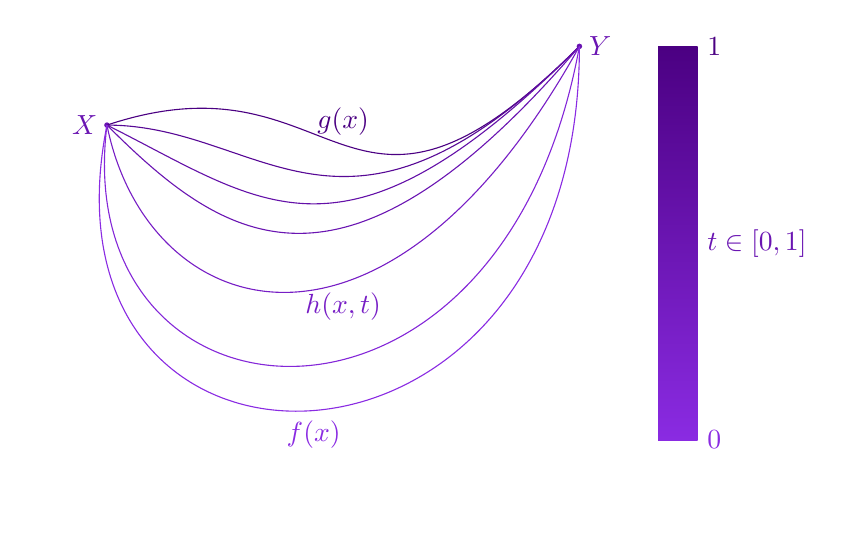
\begin{tikzpicture}
    \contourlength{1.2pt}
  %   \pgfplotsset {colormap={timemap}{rgb=(0,0,1) rgb255=(238,140,238)}};
    \pgfplotsset {colormap={timemap}{
  %     rgb255=(0,0,255)
      rgb255=(138,43,226)
  %     rgb255=(128,0,128)
      rgb255=(75,0,130)
    }};
    \definecolor{bottomcolor}{RGB}{138,43,226}
    \definecolor{topcolor}{RGB}{75,0,130}
    \tikzset{
      middlecolor/.style={
	  color of colormap={500},
	  midway,anchor=west,
      }
    }
    \begin{scope}
%     \draw[help lines] (-4,-4) grid (4,4);
    \path[fill,color of colormap={500} of timemap,left] (-3,2) circle (1pt) node {$X$};
    \path[fill,color of colormap={500} of timemap,right] (3,3) circle (1pt) node {$Y$};
    \draw[color of colormap={1000} of timemap] (-3,2) .. controls (0,3) and (0,0) .. (3,3) node[above,midway]{$g(x)$};
    \draw[color of colormap={800} of timemap] (-3,2) .. controls (-1,2) and (0,0) .. (3,3);
    \draw[color of colormap={600} of timemap] (-3,2) .. controls (-1,1) and (0,0) .. (3,3);
    \draw[color of colormap={500} of timemap] (-3,2) .. controls (-1.5,0.5) and (0,-0.5) .. (3,3);
%     \draw[color of colormap={400} of timemap] (-3,2) .. controls (-2,0) and (0,-1) .. (3,3);
    \draw[color of colormap={300} of timemap] (-3,2) .. controls (-2.5,-0.5) and (0.5,-1.5) .. (3,3);
    \path (-3,2) .. controls (-2.5,-0.5) and (0.5,-1.5) .. (3,3) coordinate[](half);
    \node[below,color of colormap={300} of timemap] (half) {$h(x,t)$};
%     \node[below,color of colormap={300} of timemap] (half) {$\vdots$};
%     \node[above,color of colormap={300} of timemap] (half) {$\vdots$};
%     \draw[color of colormap={200} of timemap] (-3,2) .. controls (-3,-1) and (1,-2) .. (3,3);
    \draw[color of colormap={100} of timemap] (-3,2) .. controls (-3.5,-2) and (2,-2.5) .. (3,3);
    \draw[color of colormap={0} of timemap] (-3,2) .. controls (-4,-3) and (3,-3) .. (3,3) node[below,midway]{$f(x)$};
    \path[shade,top color = topcolor, bottom color = bottomcolor] (4,-2) rectangle (4.5,3);
    \path[bottom color = bottomcolor] (4.5,-2) -- (4.5,3)
    node[midway,anchor=west,middlecolor]{$t \in \uint$} node[pos=0.0,anchor=west,color = bottomcolor]{$0$} node[color = topcolor,pos=1.0,anchor=west]{$1$};
    \end{scope}
  \end{tikzpicture}
\end{figure}

Alternatively, one can also view $t$ as an ``extra dimension'', where $h(x,t)$ will start from a ``basis'', the mapping $f(x)$, and be smoothly deformed along
the ``extra dimension'' $t$, until it reaches its ``top'', namely, $g(x)$.
\begin{figure}[!h]
  \centering
%   \begin{asypicture}{name=cylinder}
%     settings.outformat = "pdf";
%     settings.render = 0;
%   \end{asypicture}
\end{figure}

\textit{Two maps are said to be \textbf{homotopic} if and only if there exists a homotopy connecting them.}%
% \section{Deformation retraction}
% \section{Mapping cylinder}
\subsection{CW complexes}
\subsection{Euler characteristics}
% 
\chapter{Ordered media}
For almost all of our purposes here \textit{an \textbf{ordered
medium} can be regarded as a region of space described
by a function $f(r)$ that assigns to every point of the
region an order parameter}. The possible values of the
order parameter constitute a space known as the ordered-
parameter space (or manifold of internal states).
\section{Order parameter}
\section{Topology of defects}
\subsection{Spins confined on the plane}
\subsection{Topological quantum number}
\subsection{Uniaxial nematics on the plane}
\subsection{Three-dimensional spins confined on a plane}
\subsection{Light propagation (Gaussian mode)}
% \subsubsection{Fundamental modes}
\subsubsection{Hermite-Gaussian modes}
\subsubsection{Laguerre-Gaussian modes}
\subsection{extra}
\includepdf[pages={1}]{mapping_cyl.pdf}
% 
\end{document}
